\documentclass[]{article}
\usepackage{lmodern}
\usepackage{amssymb,amsmath}
\usepackage{ifxetex,ifluatex}
\usepackage{fixltx2e} % provides \textsubscript
\ifnum 0\ifxetex 1\fi\ifluatex 1\fi=0 % if pdftex
  \usepackage[T1]{fontenc}
  \usepackage[utf8]{inputenc}
\else % if luatex or xelatex
  \ifxetex
    \usepackage{mathspec}
    \usepackage{xltxtra,xunicode}
  \else
    \usepackage{fontspec}
  \fi
  \defaultfontfeatures{Mapping=tex-text,Scale=MatchLowercase}
  \newcommand{\euro}{€}
\fi
% use upquote if available, for straight quotes in verbatim environments
\IfFileExists{upquote.sty}{\usepackage{upquote}}{}
% use microtype if available
\IfFileExists{microtype.sty}{%
\usepackage{microtype}
\UseMicrotypeSet[protrusion]{basicmath} % disable protrusion for tt fonts
}{}
\usepackage[margin=1in]{geometry}
\usepackage{longtable,booktabs}
\usepackage{graphicx}
\usepackage{subfigure}
 \usepackage{algpseudocode} 
 \usepackage{algorithm}

\makeatletter
\def\maxwidth{\ifdim\Gin@nat@width>\linewidth\linewidth\else\Gin@nat@width\fi}
\def\maxheight{\ifdim\Gin@nat@height>\textheight\textheight\else\Gin@nat@height\fi}
\makeatother
% Scale images if necessary, so that they will not overflow the page
% margins by default, and it is still possible to overwrite the defaults
% using explicit options in \includegraphics[width, height, ...]{}
\setkeys{Gin}{width=\maxwidth,height=\maxheight,keepaspectratio}
\ifxetex
  \usepackage[setpagesize=false, % page size defined by xetex
              unicode=false, % unicode breaks when used with xetex
              xetex]{hyperref}
\else
  \usepackage[unicode=true]{hyperref}
\fi
\hypersetup{breaklinks=true,
            bookmarks=true,
            pdfauthor={},
            pdftitle={4\^{}\{th\} Report},
            colorlinks=true,
            citecolor=blue,
            urlcolor=blue,
            linkcolor=magenta,
            pdfborder={0 0 0}}
\urlstyle{same}  % don't use monospace font for urls
\setlength{\parindent}{0pt}
\setlength{\parskip}{6pt plus 2pt minus 1pt}
\setlength{\emergencystretch}{3em}  % prevent overfull lines
\setcounter{secnumdepth}{5}

%%% Use protect on footnotes to avoid problems with footnotes in titles
\let\rmarkdownfootnote\footnote%
\def\footnote{\protect\rmarkdownfootnote}

%%% Change title format to be more compact
\usepackage{titling}

% Create subtitle command for use in maketitle
\newcommand{\subtitle}[1]{
  \posttitle{
    \begin{center}\large#1\end{center}
    }
}

\setlength{\droptitle}{-2em}
  \title{Report}
  \pretitle{\vspace{\droptitle}\centering\huge}
  \posttitle{\par}
  \author{}
  \preauthor{}\postauthor{}
  \predate{\centering\large\emph}
  \postdate{\par}
  %\date{7th of July}

\DeclareMathOperator*{\argmax}{arg\,max}

\begin{document}

\maketitle

\section*{Summary}

On this report we review the theory behind the diversity-dependence model under the framework described on the introductory essay. In the later section we show results of the algorithm. To materialize this theory we  

\begin{itemize}

	\item Write MLE code for diversity-dependence model
	\item Paralellize the code
	\item Create R package
	
\end{itemize}

\section*{Overview}

We consider a phylogenetic tree, mathematicaly expressed as a set $Y = (\mathcal{T},\Upsilon)$, where $\mathcal{T}$ represent the set of branching times \footnote{that is, $t_i$ is described as the minumun time over all possible times any species could take to speciate/extinct after $t_{i-1}$}, and $\Upsilon$ has the information of the topology of the tree. The markov nature of the process means that the likelihood is exaclty the product of the conditional densities \footnote{please see the introductory esay for details}, in other words, the likelihood of the tree is then described as a multiplication of an exponenial distribution and a multinomial distribution

$$ L(\theta | Y) = \displaystyle\prod_{i}^N -\sigma_i(\theta) e^{-\sigma_i(\theta) t_i} \frac{\rho_i(\theta)}{\sigma_i (\theta)} $$
thus, the log-likelihood is
$$ l(\theta | Y) = \displaystyle\sum_{i}^N -\sigma_i(\theta) t_i + log (\rho_i(\theta)) $$


\subsection*{Diversity-dependence model}

For the simplest diversity-dependence model 

$$ \lambda_{i,j} = \lambda_0 - (\lambda_0 - \mu_0)\frac{n_i}{K}, \qquad \mu_n = \mu_0 $$ 

The MLE can be finded partialy analiticaly and partialy numerically. First we consider $\sigma_i$ and $\rho_i$ 

$$ \sigma_i  = \sum_{j=1}^{N}  \lambda_0 - (\lambda_0 - \mu_0)\frac{n_i}{K} + \mu_0 
 		 = n_i(\lambda_0 + \mu_0) - n_i^2\beta_0 $$

where $ \beta_0=\left(\frac{\lambda_0-\mu_0}{K}\right)$, and

$$\rho_i = E_i(\lambda_0 - n_i\beta_0)+(1-E_i)\mu_0$$

Here, $n_i$ is defined as the number of species at time $t_i$ and $E_i$ is a binary vector with $1$ if there was an speciation at time $t_i$ or $0$ is there was an extinction at time $t_i$. 

Thus, seeking for the MLE values, we analyze the thee equations 
$$\begin{cases} \frac{\partial l(\lambda,\beta,\mu | Y)}{\partial \lambda} = 0 \\
				\frac{\partial l(\lambda,\beta,\mu  | Y)}{\partial \beta} = 0 \\
				\frac{\partial l(\lambda,\beta,\mu  | Y)}{\partial \mu} = 0 
\end{cases} $$

Firstly, after some algebra, we find a very nice analytical solution for the extinction rate parameter
\begin{equation}
\label{mu}
 \frac{\partial l(\lambda,\beta,\mu | Y)}{\partial \mu} = 0  \Leftrightarrow \hat{u}_0 = \frac{\displaystyle\sum_{i=1}^N (1-E)}{\displaystyle\sum_{i=1}^N(n_it_i)} 
\end{equation}
Moreover, with the other two equations, we have the following system
$$\begin{cases} \displaystyle\sum_{i=1}^N \frac{E_i}{\lambda-n_i\beta} = \displaystyle\sum_{i=1}^N n_i t_i \\ \displaystyle\sum_{i=1}^N \frac{E_in_i}{\lambda-n_i\beta} = \displaystyle\sum_{i=1}^N n^2_i t_i \end{cases}$$

A numerical efficient method to solve this system is described in the appendix.

\section*{Algorithm}

Under the previous results, we developed an algorithm able to find accurate solution for the MLE. The algorithm is based on the following formulation. 

Step 1. get $\hat{\mu_0}$ using eq \ref{mu}. \\
Step 2. Consider the function 

$$ \hat{\beta}(\lambda) = \displaystyle\argmax_{\beta} L(\lambda,\beta,\hat{\mu}_0) $$
\\
Step 3. Calculate the MLE such that, 


$$ (\hat{\lambda},\hat{\beta},\hat{\mu}) =  \displaystyle\argmax_{\lambda}L(\lambda,\hat{\beta}(\lambda),\hat{\mu}) $$

Two important properties of this algorithm ensures convergence (the writting of the proof is pending): 

\begin{enumerate}
	\item $ \hat{\beta}(\lambda)$ is a linear function of $\lambda$
	\item $\displaystyle\argmax_{\lambda}L(\lambda,\hat{\beta}(\lambda),\hat{\mu})$ is a convex funcion of $\lambda$.
\end{enumerate}

This two results ensures the existence of an unique global maximum, which is easily calculated by several classic optimization methods.

As an example, on figure \ref{hists} we can see the estimations over 1000 simulations of the diversity-dependence process with true values $\lambda_ = 0.8, \beta_0 = 0.0175, \mu_0 = 0.1, K=40$ and crown time $=15$. We can see accurate estimations to the true value. 
\section*{Results}
%
%\begin{table}[]
%\centering
%\caption{My caption}
%\label{my-label}
%\begin{tabular}{l|llll} \hline
%       & 1st Qu. & 2nd Qu. & 3rd Qu &  \\ \hline
%$\lambda$ & 0.748   & 0.835   & 0.928  &  \\
%$\beta$   & 0.0162  & 0.0185  & 0.0209 &  \\
%$\mu$     & 0.09    & 0.1     & 0.11   &  \\
%$K$      & 38.82   & 39.87   & 40.95  & 
%\end{tabular}
%\end{table}
On table \ref{alg} we can see the bias and precision of the maximum-likelihood estimates, as shown by the median and the 25th and 75th percentiles of the estimated parameters of 100 simulated datasets. There we can see that the results are quite accurate regarding the real values. \\

Morever, on table \ref{ddd} we have the estimated parameters of the diversity-dependence model simulated under the DDD package. Here we can see that the algorithm is even able to capture true values simulated under the DDD framework. 

\begin{table}[h!]
\centering

\caption{MLE estimation of 100 simulations. Simulations and estimations are from the algorithm described above.}
\label{alg}
\begin{tabular}{cccc|ccc@{\hskip 0.3in}ccc@{\hskip 0.3in}ccc}
\hline
\multicolumn{4}{c}{Simulated Parameters} & \multicolumn{9}{c}{Estimated parameters (25th, 50th, 75th percentiles)} \\ \hline
$\lambda_0$    & $K$     & crown age    & $\mu$    &        & $\lambda_0$  &       &       & $\mu$   &      &       & $K$     &        \\
          &       &              &       & 025th  & 50th    & 75th  & 025th & 50th & 75th & 025th & 50th  & 75th   \\
          &       &              &       &        &         &       &       &      &      &       &       &        \\
0.8       & 40    & 5            & 0     & 0.71   & 0.87    & 1.04  & 0.00  & 0.00 & 0.00 & 31.20 & 39.09 & 440.16 \\
          &       &              & 0.1   & 0.76   & 0.92    & 1.11  & 0.07  & 0.10 & 0.13 & 22.23 & 32.65 & 65.39  \\
          &       &              & 0.2   & 0.80   & 0.96    & 1.28  & 0.13  & 0.19 & 0.26 & 12.74 & 31.76 & 83.12  \\
          &       &              & 0.4   & 1.05   & 1.23    & 1.55  & 0.27  & 0.36 & 0.44 & 7.00  & 17.61 & 30.58  \\
          &       &              &       &        &         &       &       &      &      &       &       &        \\
          &       & 10           & 0     & 0.68   & 0.79    & 0.87  & 0.00  & 0.00 & 0.00 & 39.63 & 40.98 & 43.92  \\
          &       &              & 0.1   & 0.71   & 0.86    & 0.98  & 0.09  & 0.10 & 0.12 & 37.11 & 39.52 & 42.01  \\
          &       &              & 0.2   & 0.78   & 0.91    & 1.05  & 0.18  & 0.20 & 0.23 & 34.08 & 38.13 & 43.32  \\
          &       &              & 0.4   & 0.87   & 1.01    & 1.20  & 0.37  & 0.41 & 0.46 & 18.32 & 30.13 & 42.13  \\
          &       &              &       &        &         &       &       &      &      &       &       &        \\
          &       & 15           & 0     & 0.69   & 0.77    & 0.87  & 0.00  & 0.00 & 0.00 & 39.58 & 40.00 & 41.03  \\
          &       &              & 0.1   & 0.72   & 0.80    & 0.91  & 0.09  & 0.10 & 0.11 & 38.72 & 39.89 & 40.98  \\
          &       &              & 0.2   & 0.78   & 0.84    & 0.96  & 0.18  & 0.20 & 0.22 & 38.29 & 40.25 & 41.93  \\
          &       &              & 0.4   & 0.79   & 0.90    & 1.00  & 0.38  & 0.40 & 0.43 & 31.40 & 37.38 & 43.89 
\end{tabular}
\end{table}



 \begin{figure}[h]
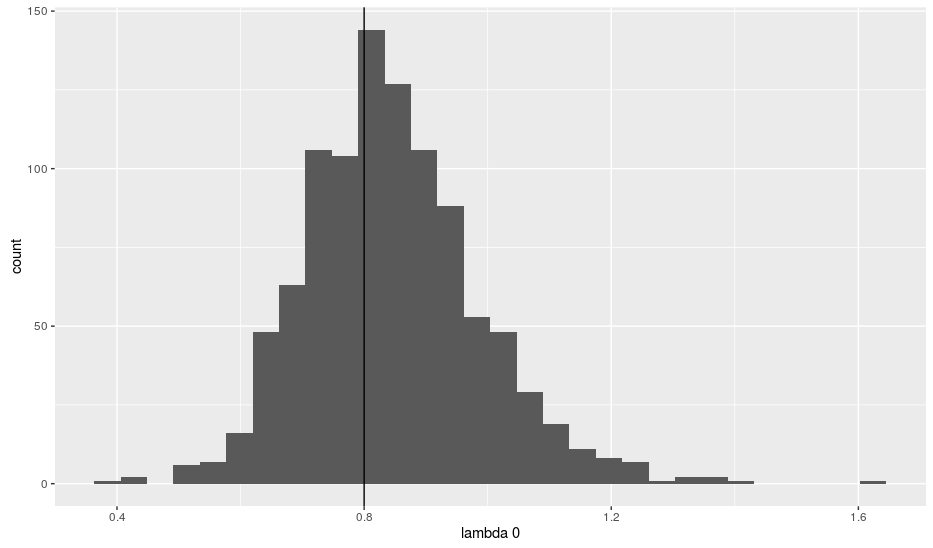
\includegraphics[width=.5\textwidth]{lambda.png}
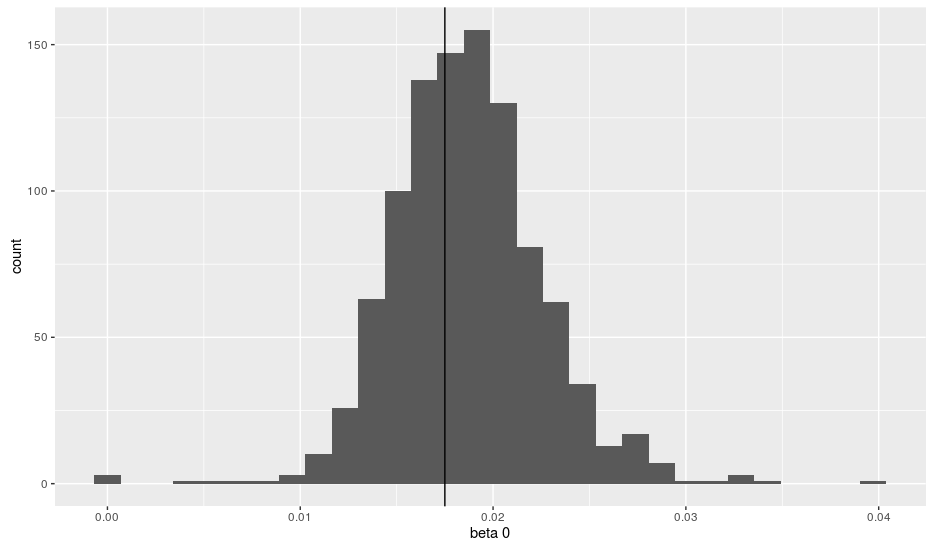
\includegraphics[width=.5\textwidth]{beta.png}
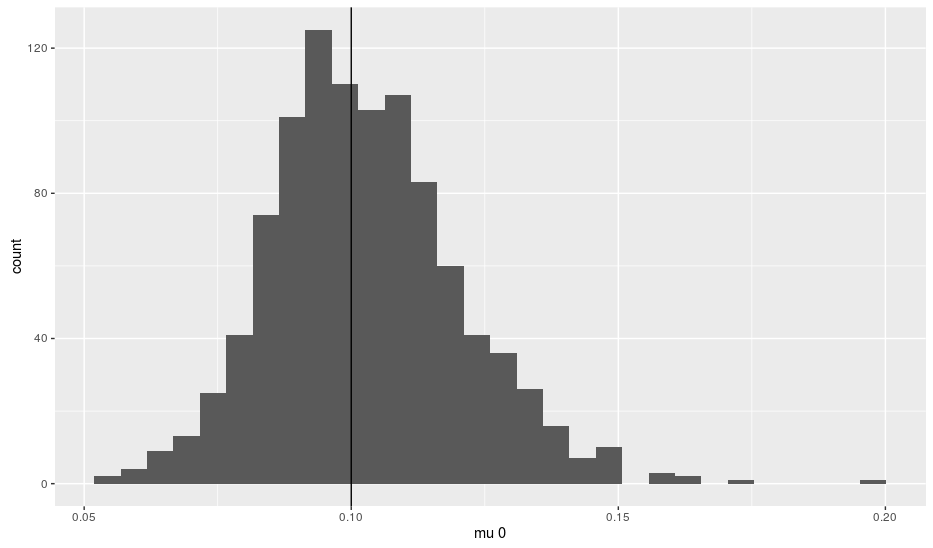
\includegraphics[width=.5\textwidth]{mu.png}
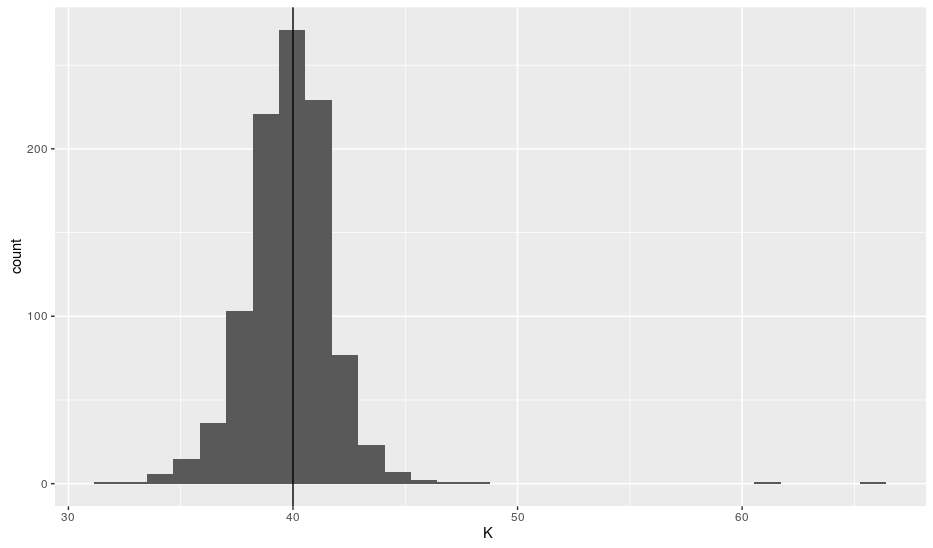
\includegraphics[width=.5\textwidth]{K.png}
%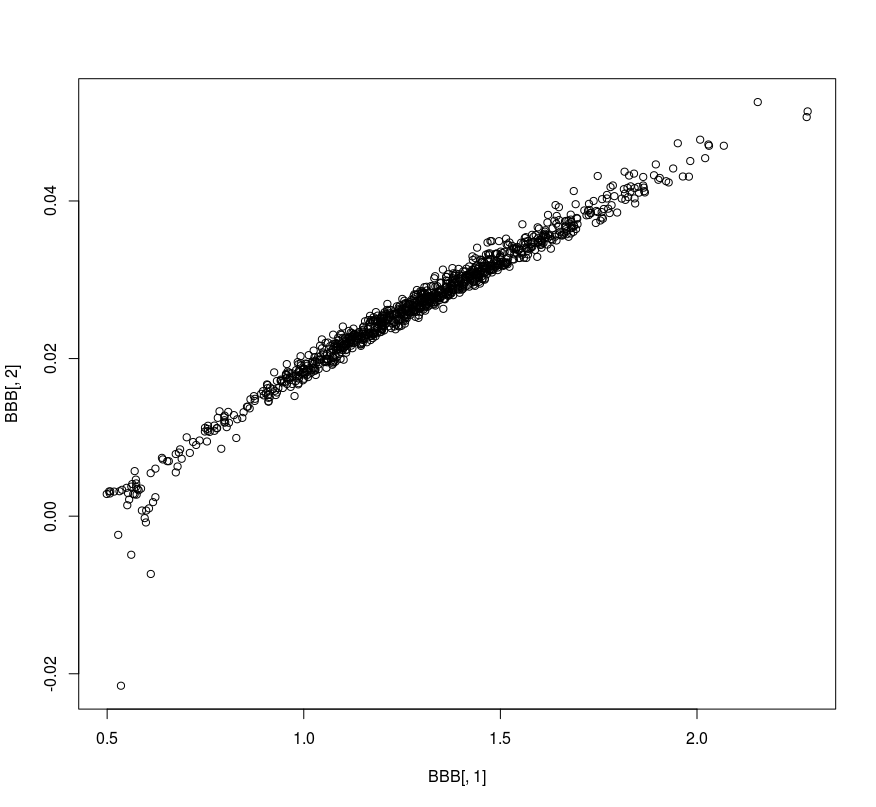
\includegraphics[width=.5\textwidth]{bolh.png}
%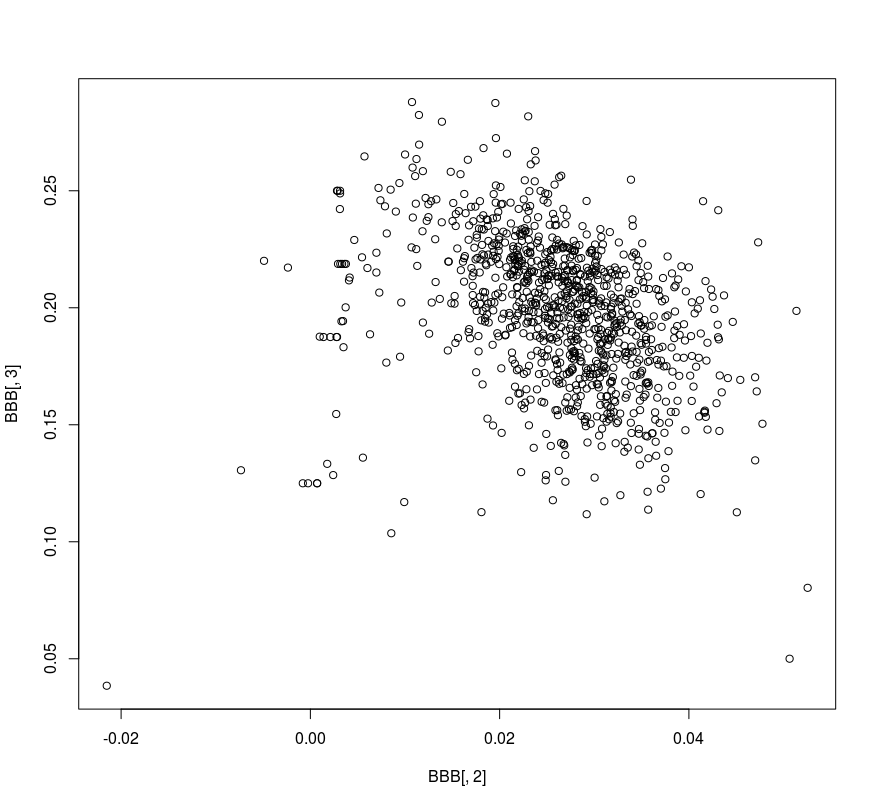
\includegraphics[width=.5\textwidth]{b0mh.png}
\label{hists}
\caption{Estimations over 1000 simulations of the diversity-dependence process with true values $\lambda_ = 0.8, \beta_0 = 0.0175, \mu_0 = 0.1, K=40$ and crown time $=15$. The black vertical lines shows the real values.}
\end{figure}


\begin{table}[h!]
\centering

\caption{MLE estimation of 100 simulations. Simulations are from the 'DDD' package and estimation from p1 algorithm.}
\label{ddd}
\begin{tabular}{cccc|ccc@{\hskip 0.3in}ccc@{\hskip 0.3in}ccc}
\hline
\multicolumn{4}{c}{Simulated Parameters} & \multicolumn{9}{c}{Estimated parameters (25th, 50th, 75th percentiles)} \\ \hline
        &       &              &        &         &       &       &        &       &       &       &       &       \\
$\lambda_0$     & $K$     & crown age    & $\mu$     &   &  $\lambda_0$     &       &      &  $\mu$     &       &      &  $K$     &       \\
%           &       &              &        & 025th   & 50th  & 75th  & 025th  & 50th  & 75th  & 025th & 50th  & 75th  \\
   
0.8        & 40    & 5            & 0      & 0.74    & 0.91  & 1.11  & 0.00   & 0.00  & 0.00  & 34.84 & 41.04 & 59.34 \\
           &       &              & 0.1    & 0.94    & 1.15  & 1.28  & 0.08   & 0.11  & 0.14  & 26.57 & 32.55 & 39.98 \\
           &       &              & 0.2    & 1.03    & 1.22  & 1.46  & 0.17   & 0.21  & 0.29  & 17.06 & 27.85 & 37.47 \\
           &       &              & 0.4    & 1.13    & 1.43  & 1.67  & 0.33   & 0.42  & 0.52  & 9.40  & 17.52 & 27.29 \\
           &       &              &        &         &       &       &        &       &       &       &       &       \\
           &       & 10           & 0      & 0.75    & 0.87  & 0.98  & 0.00   & 0.00  & 0.00  & 38.55 & 39.33 & 40.35 \\
           &       &              & 0.1    & 0.78    & 0.90  & 1.05  & 0.09   & 0.10  & 0.12  & 37.09 & 38.55 & 40.33 \\
           &       &              & 0.2    & 0.86    & 0.96  & 1.08  & 0.19   & 0.21  & 0.23  & 34.47 & 37.45 & 40.38 \\
           &       &              & 0.4    & 0.96    & 1.11  & 1.22  & 0.38   & 0.42  & 0.45  & 28.11 & 33.88 & 40.41 \\
           &       &              &        &         &       &       &        &       &       &       &       &       \\
           &       & 15           & 0      & 0.74    & 0.83  & 0.96  & 0.00   & 0.00  & 0.00  & 38.57 & 39.05 & 40.00 \\
           &       &              & 0.1    & 0.80    & 0.88  & 0.99  & 0.09   & 0.11  & 0.12  & 37.57 & 38.67 & 39.57 \\
           &       &              & 0.2    & 0.88    & 0.95  & 1.05  & 0.20   & 0.21  & 0.22  & 36.98 & 38.58 & 40.07 \\
           &       &              & 0.4    & 0.92    & 1.03  & 1.14  & 0.38   & 0.41  & 0.44  & 34.02 & 37.45 & 41.96
\end{tabular}
\end{table}


%
%\subsection*{Parallelization}
%
%Bellow we can see the table with the corresponding time
%
%\section*{Package}
%
%The 'unnamed' package holds the following functions
%
%\begin{itemize}
%
%	\item
%
%\end{itemize}
%
%\section*{Further steps}
%
%to do: 

\section*{Further steps: First Ideas about MCEM applied to incomplete phylogenies}

To complete this first example we would like to estimate trees where extinc species are not observable. Bellow is a draft of the pseudo-code, inspired on a montecarlo EM algorithm approach.\\

\begin{algorithm}
\caption{Montecarlo EM aproach}
\label{mcem}
\begin{algorithmic}[1]
\State Set number of iterations, initial parameters
\Repeat
\For {$i$ in 1:nit} \\
\qquad simulate a reconstructed phylogenetic tree with algorithm \ref{euclid}\\
\qquad use the simulated tree to estimate parameters 
\EndFor \\
average parameters and use it as initial parameters\\
\Until{convergence}
 
\end{algorithmic}
\end{algorithm}




\begin{algorithm}
\caption{simulation of a reconstructed tree}
\label{euclid}
\begin{algorithmic}[1]
%\caption{Montecarlo EM aproach}\label{euclid}
\State Load the incomplete phylogenetic tree
\State set $t$ be the vector of branching times of the incomplete tree
\For {$i$ in 1:length(t)} \\
\quad	update $\lambda$ and $\mu$ for moment $t_i$ \\
\quad	simulate a new branching time $t_{temp}$ from $t_i$ 
	\While {$t_{temp}<t_{i+1}$} \\
	 \qquad	simulate the extinction event from exponential distribution with rate $\mu_{i}$\\
	 \qquad	simulate new branching time $t_{temp}$ from previous $t_{temp}$ and extinction event\\
	\qquad	update $\lambda$ and $\mu$ for moment $t_i$
	\EndWhile\\
	update the reconstructed tree
\EndFor \\
\Return Reconstructed tree
 
\end{algorithmic}
\end{algorithm}

\newpage
\section*{Appendix}


In order to solve the system given by the diversity-dependence set up we consider the following idea,\\

Given 

\begin{itemize}
	\item $b_1, b_2, \dots, b_n \in \{0,1\}$
	\item $m_1, m_2, \dots, m_n \in \mathbb N$
	\item $c_1, c_2 \in \mathbb R$
\end{itemize}


define  

$$ z_i := \dfrac{1}{\lambda - m_i \beta} $$

we have a system of $2$ equaions in $\mathrm z \in \mathbb R^n$

$$ \begin{bmatrix} b_1 & b_2 & \dots & b_n\\ b_1 m_1 & b_2 m_2 & \dots & b_n m_n\end{bmatrix} \begin{bmatrix} z_1\\ z_2\\ \vdots\\ z_n\end{bmatrix} = \begin{bmatrix} c_1\\ c_2\end{bmatrix}$$

or, in a more succinct form, $\mathrm A \mathrm z = \mathrm c$. If $n>2$, this is an underdetermined system whose {\bf least-norm} solution is 

$$\hat{\mathrm z} := \mathrm A^T (\mathrm A \mathrm A^T)^{-1} \mathrm c$$

If all the entries of $\hat{\mathrm z}$ are nonzero, then we have an overdetermined system of equations 

 $$ \begin{array}{rl} x - m_1 y &= \hat z_1^{-1}\\ x - m_2 y &= \hat z_2^{-1}\\ &\vdots \\ x - m_n y &= \hat z_n^{-1}\end{array} $$
 
 Lastly, we compute the {\bf least-squares} solution $(\hat \lambda, \hat \beta)$. If $\hat z_i = 0$, then the $i$-th equation, whose right-hand side is illegal, is simply discarted. 

\end{document}
